\documentclass[manuscript,screen,nonacm]{acmart}
\setcopyright{none}
\settopmatter{printacmref=false,printccs=false}
\acmDOI{}
\acmISBN{}
\usepackage{graphicx,xurl,placeins}
\setcitestyle{numbers}
\raggedbottom
\title{ARC Explorer: A Native macOS Workspace for Remote High-Performance Computing}
\subtitle{Technical report; ARC Explorer v0.1; November 13, 2026.}
\author{William Taggart}
\affiliation{\department{Modern and Classical Languages and Literatures}\institution{Virginia Tech}\city{Blacksburg}\state{Virginia}\country{USA}}
\email{wtaggart@vt.edu}

% Permit figures to share pages with surrounding explanatory text.
\renewcommand{\topfraction}{0.92}
\renewcommand{\bottomfraction}{0.85}
\renewcommand{\textfraction}{0.06}
\renewcommand{\floatpagefraction}{0.80}
\setcounter{topnumber}{3}
\setcounter{bottomnumber}{3}
\setcounter{totalnumber}{5}
\setlength{\textfloatsep}{12pt plus 2pt minus 3pt}
\setlength{\intextsep}{12pt plus 2pt minus 3pt}
\raggedbottom

\geometry{top=0.65in,bottom=0.55in,includeheadfoot}
\begin{document}
\begin{abstract}
ARC Explorer is a native macOS application that brings connection profiles, resource inspection, allocation accounting, GPU job submission, remote files, terminal sessions, web applications, and language-model assistance into one workspace for Virginia Tech Advanced Research Computing (ARC). The client combines SwiftUI, AppKit, WebKit, the system SSH client, and a small remote Python helper. Computational scripts are submitted to Slurm with explicit resource requests, while an integrated login-node terminal supports direct interactive administration. Five main sections organize the workflow: Connection, Resources, Jobs + software, Sessions, and Help. This report describes the implementation, file-editing safeguards, credential boundaries, installation workflow, and release validation. Twenty-eight Python tests and two native terminal tests pass for the release candidate. The evidence establishes functional checks of selected paths, not a performance benchmark, independent security audit, or guarantee of compatibility with every ARC service. Five application screenshots illustrate the workspace.
\end{abstract}
\keywords{high-performance computing, Slurm, SSH, macOS, scientific gateways, remote development}
\maketitle

\section{Motivation and context}

Researchers using a shared cluster must coordinate several interfaces: SSH authentication, scheduler commands, allocation and storage reports, source repositories, text editors, interactive notebooks, and service documentation. ARC Explorer groups these operations around a saved cluster profile and an explicit resource request. The goal is to reduce interface switching while keeping the underlying commands, execution locations, and resource decisions visible.

Web gateways already provide broad access to high-performance computing. Open OnDemand is an established portal architecture for HPC centers \cite{hudak2018}, and ARC documents its deployment for files, jobs, shells, and interactive applications \cite{arcood}. ARC Explorer complements that infrastructure with a native desktop workspace, an embedded browser, a terminal, and local document dialogs. It does not replace the scheduler, identity provider, allocation service, or Open OnDemand deployment. No comparative usability advantage is asserted.

The scheduler remains the authority on resource allocation. Slurm exposes submission, queue inspection, accounting, and cancellation through established commands \cite{slurm}. The application translates form values into explicit scheduler arguments rather than implementing its own queue. ARC's login-node guidance constrains the intended use of interactive commands \cite{arcpolicy}. The distinction between management and compute is therefore part of both the interface and the implementation, although the general terminal cannot enforce that distinction.

\subsection{Research context}

The original Slurm paper describes resource management and scheduling as services of the cluster infrastructure \cite{slurmpaper}. This provides the architectural basis for keeping a desktop client's resource form separate from the scheduler that grants and enforces an allocation. A submitted request is therefore an auditable specification of desired resources, not proof of their availability.

Research on Jupyter notebooks treats executable code, results, and explanatory prose as a shared publication artifact \cite{notebooks}. ARC Explorer's embedded notebook access supports that workflow, while the notebook server and compute allocation retain their own lifecycles. Peng's account of reproducible computational research emphasizes access to the computational artifacts needed to inspect a result \cite{repro}. The FAIR principles additionally distinguish findability, accessibility, interoperability, and reuse \cite{fair}. These perspectives motivate saving scripts, resource settings, environment information, and outputs together. They do not establish that a GUI, a saved script, or an exported log by itself makes an experiment reproducible or FAIR-compliant.

\section{Architecture and execution boundaries}

The desktop application targets Apple Silicon Macs running macOS 15 or later. SwiftUI provides the workspace and forms; AppKit supplies native dialogs and terminal integration; WebKit renders web services. The application calls the macOS system SSH executable. It does not require a separately installed local Python interpreter, browser engine, or model weights. A system browser remains available as an alternative for web authentication and applications.

SSH establishes a reusable authenticated control connection. Structured management requests invoke the bundled remote helper through SSH using Python 3 on the remote host. The helper uses Python's standard library, returns JSON, and does not install a persistent daemon or request elevated privileges. Remote Python is therefore a runtime dependency even though local Python is not. Scheduler commands, file operations, and short discovery queries execute under the authenticated user's permissions.

The implementation has three distinct execution paths. First, bounded management requests run on the login host. Second, submitted scripts run under a Slurm allocation on the assigned compute node. Third, the user-controlled terminal opens an interactive login-node shell. The ARC LLM assistant is a separate HTTPS client; it does not reuse SSH credentials. Embedded web pages have their own authentication and service lifecycle.

The remote helper is itself a Python process on the login node. ARC's published guidance is restrictive about Python use there \cite{arcpolicy}. Its use for bounded management operations should not be interpreted as institutional approval or as an exemption from site policy. The application does not perform inference or package installation through that helper. General terminal commands remain the user's responsibility.

Nonsecret connection preferences, appearance, bookmarks, and workspace state are stored locally. Profiles contain connection and resource settings, not SSH passwords or private-key material. The local workspace preserves drafts for convenience; it is not a transaction log or a substitute for saving important scripts and files.

\section{Connection: profiles and authentication}

The Connection section presents saved profiles, host and port fields, a Virginia Tech PID, authentication mode, private-key path, and remote workspace location. Presets cover TinkerCliffs, Falcon, and Owl; a custom host can be entered. The selected profile also carries the account and resource preferences used by subsequent jobs. A preset is a convenience, not evidence that the host or a GPU partition is currently available.

Authentication supports an SSH key or agent and password plus Duo. A native askpass helper displays SSH authentication prompts. Passwords, private-key passphrases, and Duo responses are not serialized into settings. The client preserves SSH host-key verification and asks when a host key needs acceptance. Hostnames, user names, and ports are validated before command construction.

The reusable SSH control socket is placed in a private temporary directory. Multiplexing avoids repeating a full authentication exchange for every small management request. Disconnecting closes the client connection; it does not cancel already submitted Slurm jobs. Switching profiles requires disconnecting first so that a visible cluster profile does not silently refer to a different active connection.

Light mode is the default, with an explicit dark-mode option. The header uses a bold ARC wordmark and a lighter Explorer wordmark. A resource library and current GPU-request summary provide context across sections. The interface keeps progress and connection state visible without claiming that a queued request is already computing.

\begin{figure}[!htb]
\centering
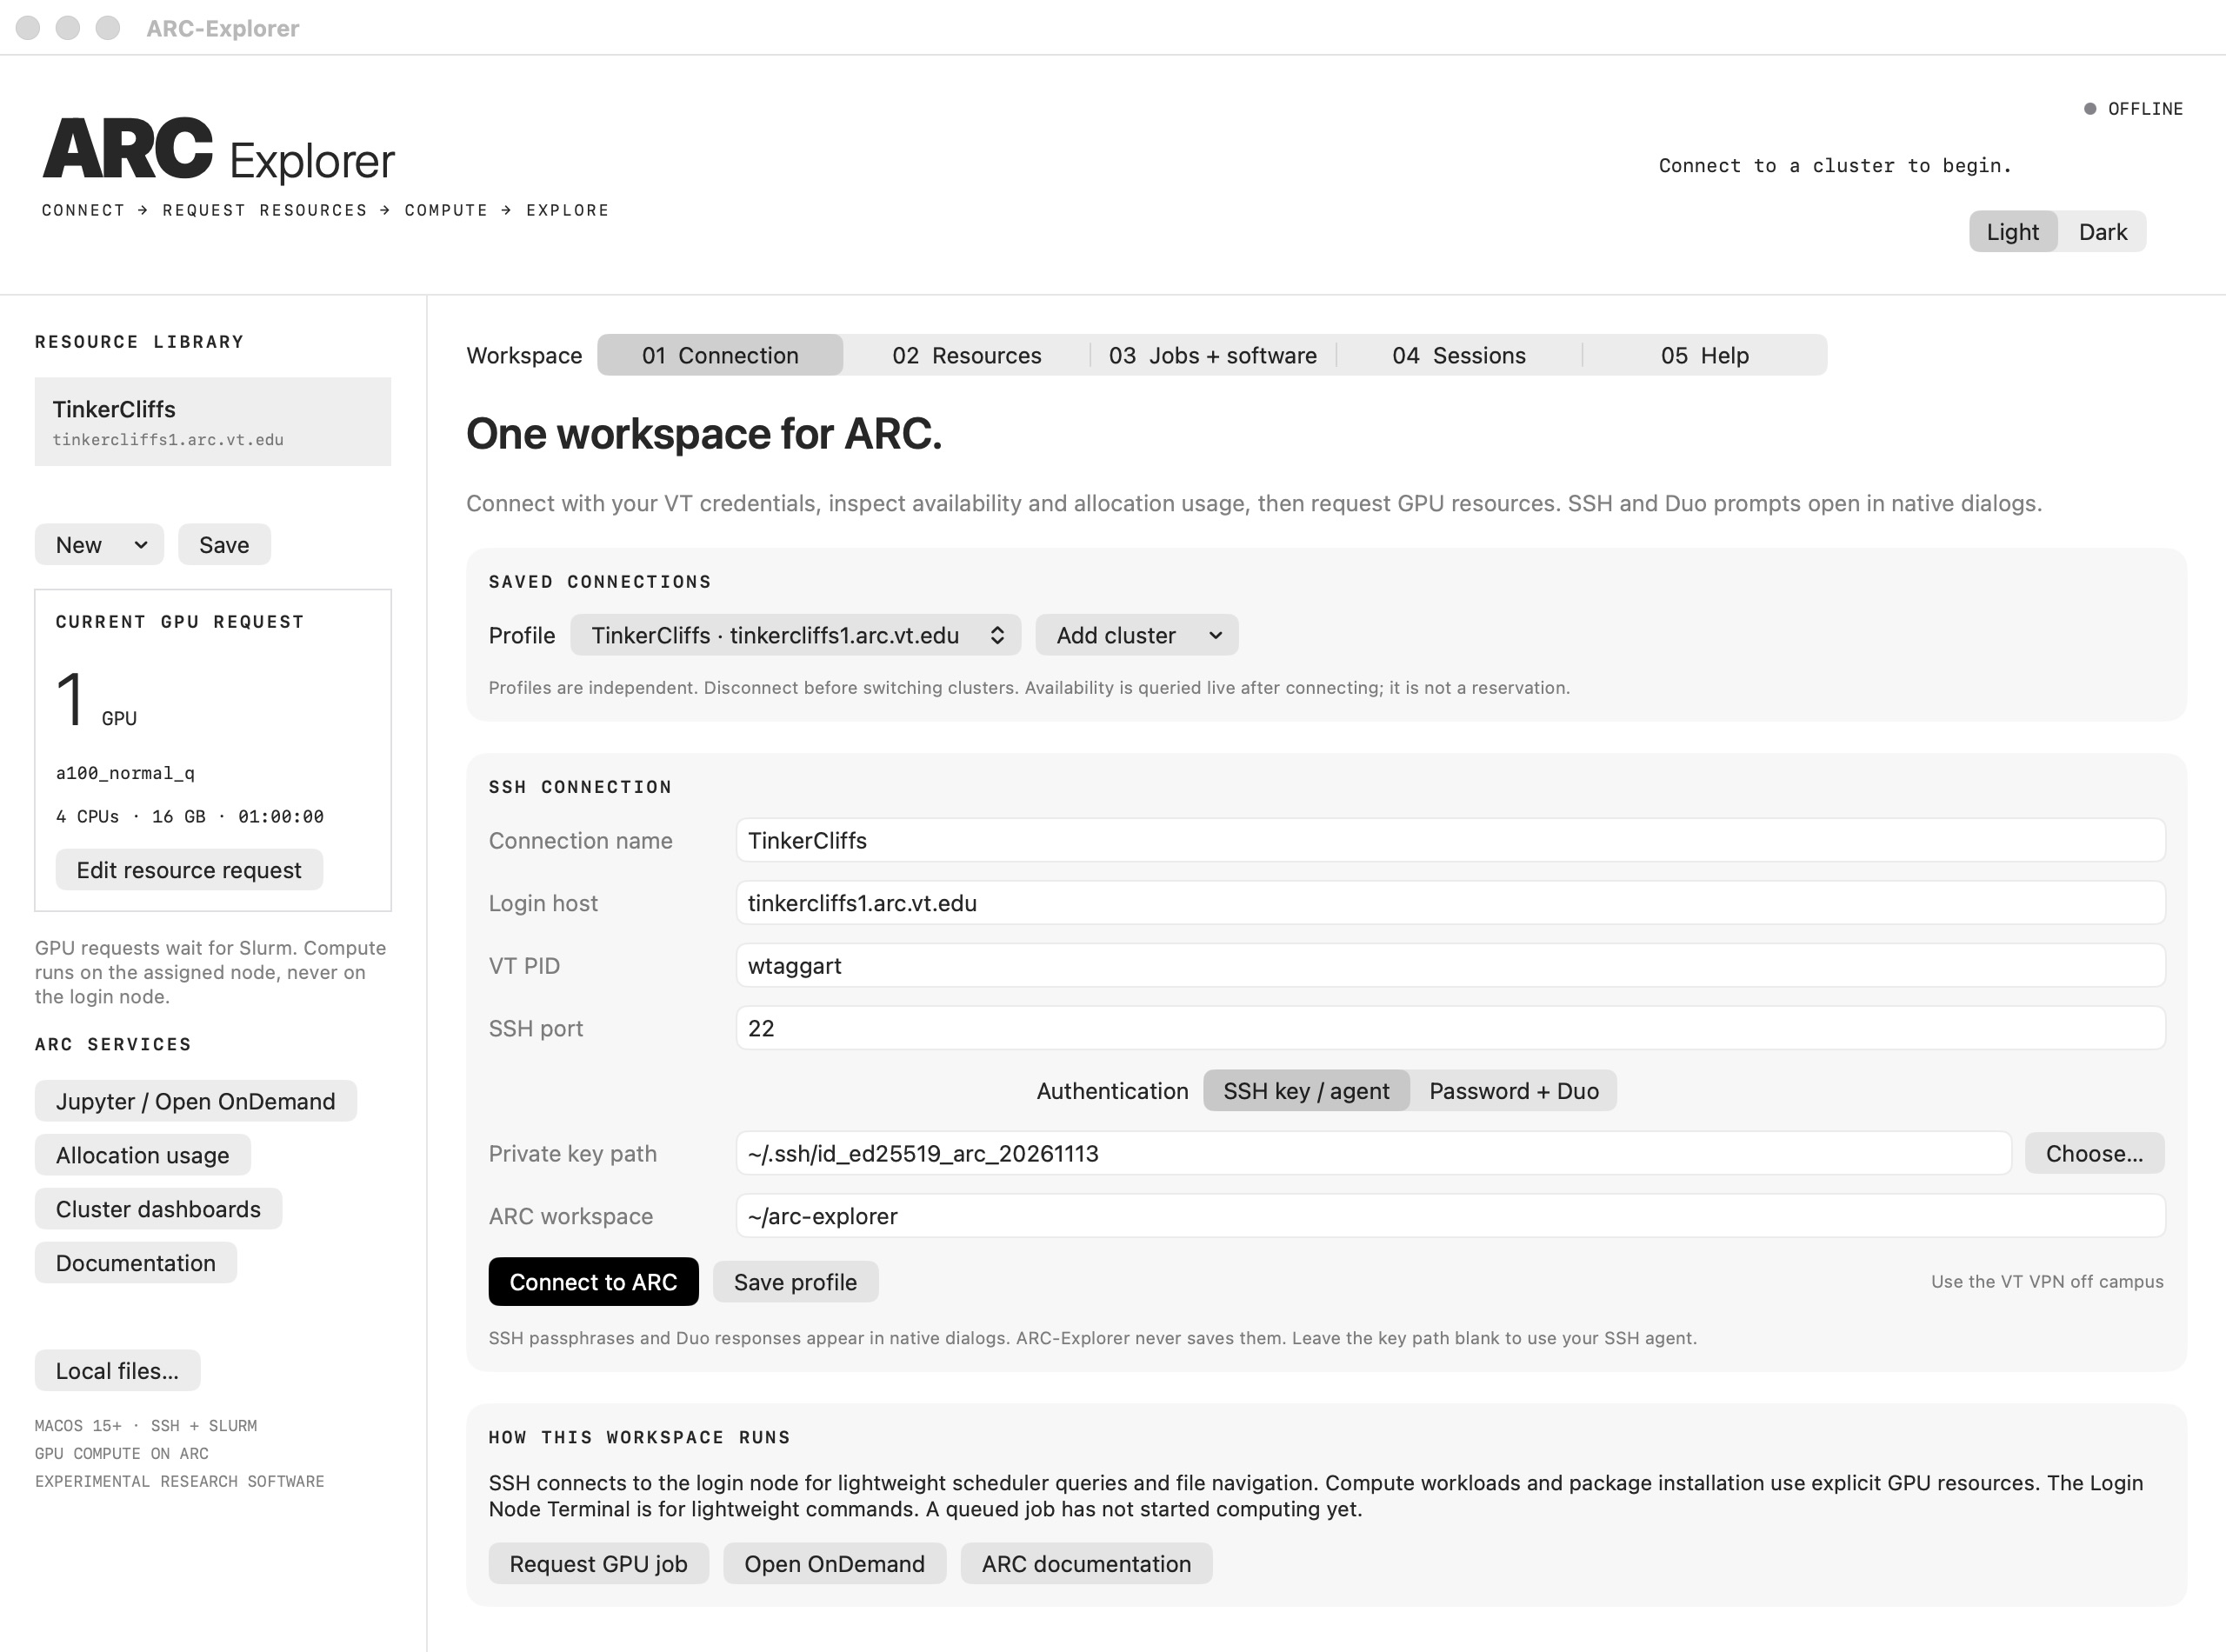
\includegraphics[width=0.78\textwidth,height=0.62\textheight,keepaspectratio]{figures/01-connection.png}
\caption{Connection section showing the saved profile and SSH form. Offline capture of the signed v0.1 build; no password, API key, or private-key contents are shown.}
\Description{Connection section showing the saved profile and SSH form. Offline capture of the signed v0.1 build; no password, API key, or private-key contents are shown.}
\end{figure}

\section{Resources: availability, accounting, and remote files}

Availability queries inspect cluster partitions, user associations, and storage information through the connected host. The application also opens ARC's all-cluster dashboards at the kiosk dashboard URL. These observations describe current or reported state; they neither reserve capacity nor predict queue time.

Allocation usage combines ARC's getusage and quota reports with Slurm accounting and fair-share information. The user specifies an allocation and a date range for the job table. Site allocation and quota reports retain their own reporting periods. Slurm fair-share usage is explicitly distinguished from a remaining allocation balance. Account-wide visibility depends on the user's permissions. Reports are captured independently so that one unavailable command does not erase other useful results.

The Remote files view lists directories, supports folder creation, and uploads or downloads bounded files. Listings are limited to 5,000 entries, and transfers are capped at 8 MiB per file in this version. Upload creation is exclusive: an existing destination is not silently replaced. These are interactive convenience operations rather than a bulk data-transfer system.

The lightweight editor opens UTF-8 text files up to 1 MiB, supports new files and reload, and saves through a native action or Command-S. Its conservative save path accepts regular files owned by the user and rejects symbolic links, hard links, special files, binary or invalid UTF-8 content, and files with unsupported extended metadata. Unsaved edits trigger a warning before replacement or application exit. Editing state persists across workspace navigation, but unsaved edits should not be treated as crash-resistant storage.

An opened file is associated with a revision derived from its content hash, device, inode, and modification time. Before replacement, the helper compares the current revision with the expected revision, writes a temporary file in the destination directory, preserves supported permissions and group metadata, flushes it, checks again, and replaces the destination. A detected conflict preserves the remote version. This is optimistic conflict detection; it is not a server-side lock or a proof that all concurrent-writer races are impossible.



\begin{figure}[!htb]
\centering
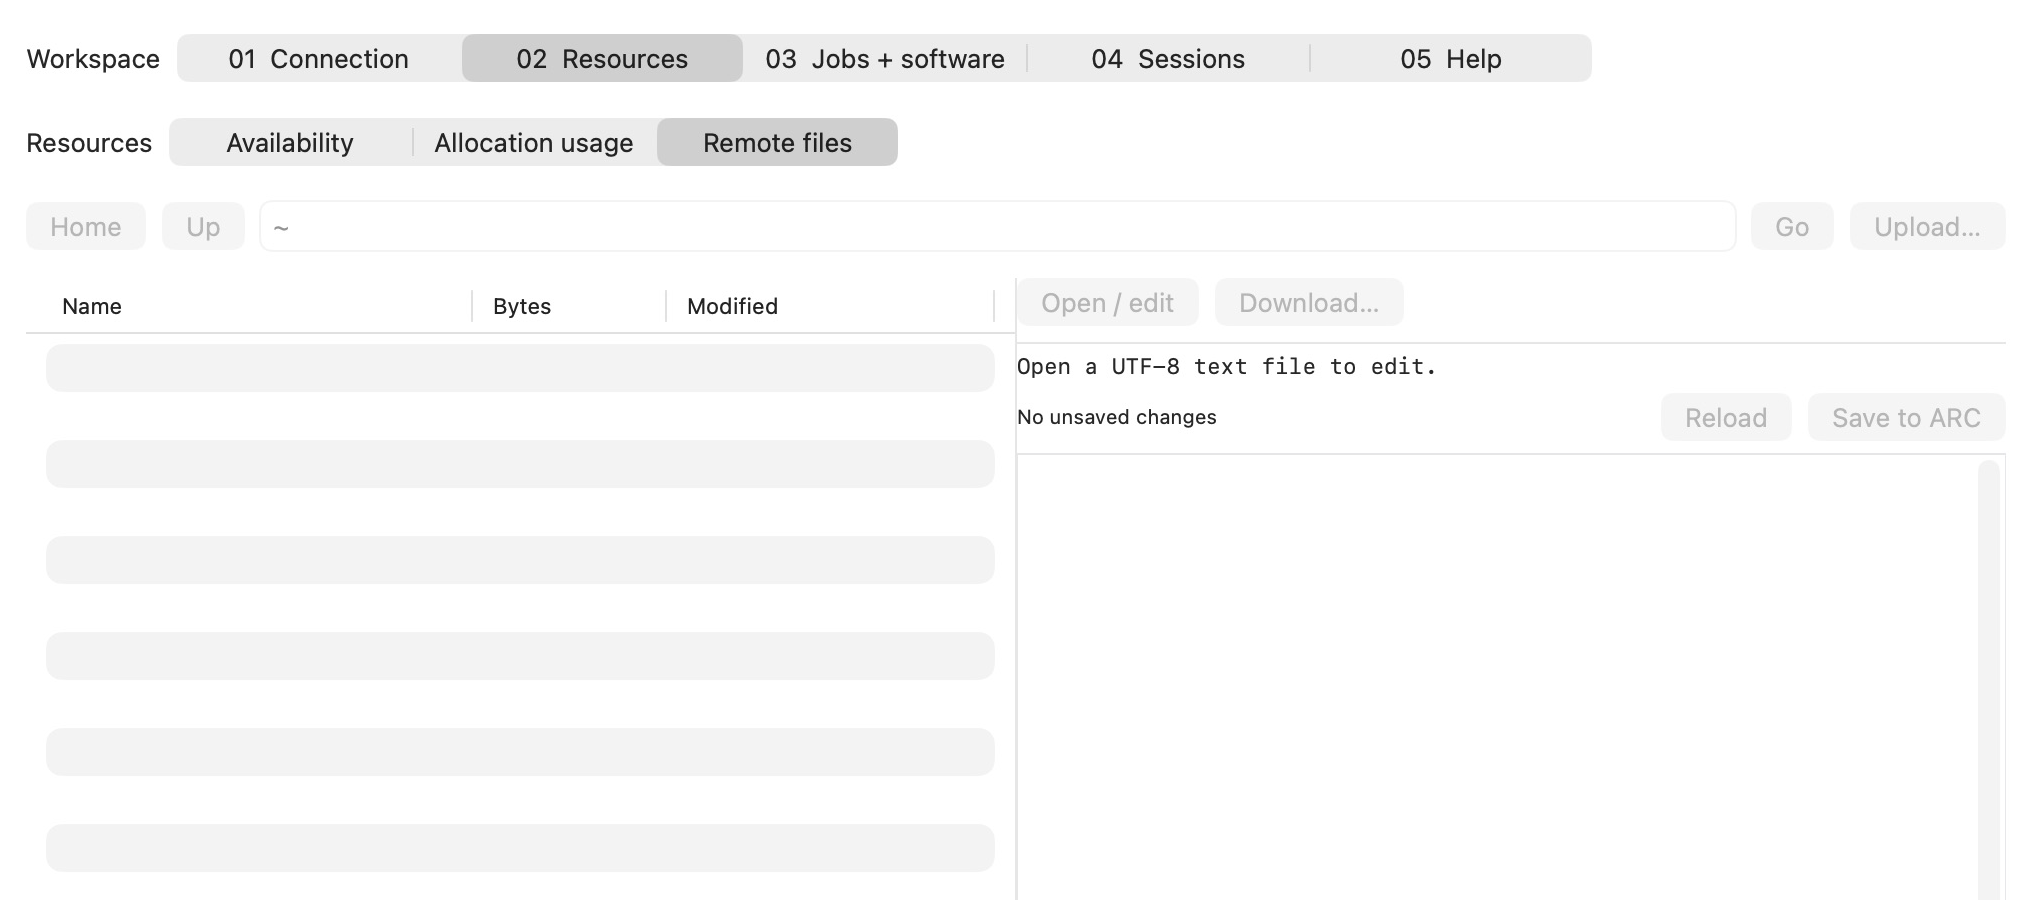
\includegraphics[width=0.78\textwidth,height=0.62\textheight,keepaspectratio]{figures/06-file-editor.png}
\caption{Cropped detail of the remote file browser and lightweight text editor. This offline view illustrates the editing controls, not an active file transaction.}
\Description{Cropped detail of the remote file browser and lightweight text editor. This offline view illustrates the editing controls, not an active file transaction.}
\end{figure}

\section{Jobs + software: resource requests and reproducible scripts}

The GPU request form exposes allocation, partition, wall time, GPU count, CPU count, memory, and working directory. Version 0.1 accepts one to eight GPUs, one to 256 CPUs, and one to 2,048 GiB-equivalent Slurm memory units expressed with the G suffix. These are client validation bounds, not promises that a partition supports every combination. Users must choose values allowed by their account and the selected partition.

Submission creates a per-job directory with a UUID, a shell script, job metadata, and a log destination. The helper submits the script with sbatch, requests one node and one task, and passes the allocation, partition, time, CPUs, memory, GPU generic resource, working directory, and log arguments explicitly. The shell wrapper uses strict error handling. Script content is limited to 200,000 UTF-8 bytes. A confirmation precedes submission. Saving a script does not execute it.

Users can open an existing script, edit it, and save it either on the Mac or on ARC. The reusable script file and the resource form are separate: saving the text does not embed all resource settings in scheduler directives. This distinction lets one script be reused with different allocations but requires users to preserve resource choices separately when reproducing a run outside the app.

Jobs + results provides queue and accounting views, pending reasons, details, logs, and cancellation for the user's jobs. Automatic refresh runs every 30 seconds while the connected Jobs view is active and idle. The remote cancellation path verifies ownership. Jobs continue in Slurm after the Mac disconnects or the application closes. Reconnection and accounting, rather than the GUI process lifetime, determine how their results are recovered.

Install / update code generates a reviewable script for a GitHub or Hugging Face owner/repository pair. The script clones into a dedicated destination or checks an existing checkout for the expected origin and a clean working tree before updating. Ordinary updates use fast-forward-only behavior; an explicit revision can be checked out detached. Hugging Face retrieval requires Git LFS on the remote host. Local GitHub and Hugging Face credentials are not automatically copied to ARC.

Repository retrieval does not automatically run arbitrary setup instructions. The user reviews the generated script, adds needed modules or environment steps, and submits it as a GPU job. Private repositories require suitable remote credentials. The module-discovery controls and command reference help identify available toolchains. The native form is GPU-oriented; a general CPU-only resource form, job arrays, and multi-node configuration are not implemented in v0.1.

\begin{figure}[!htb]
\centering
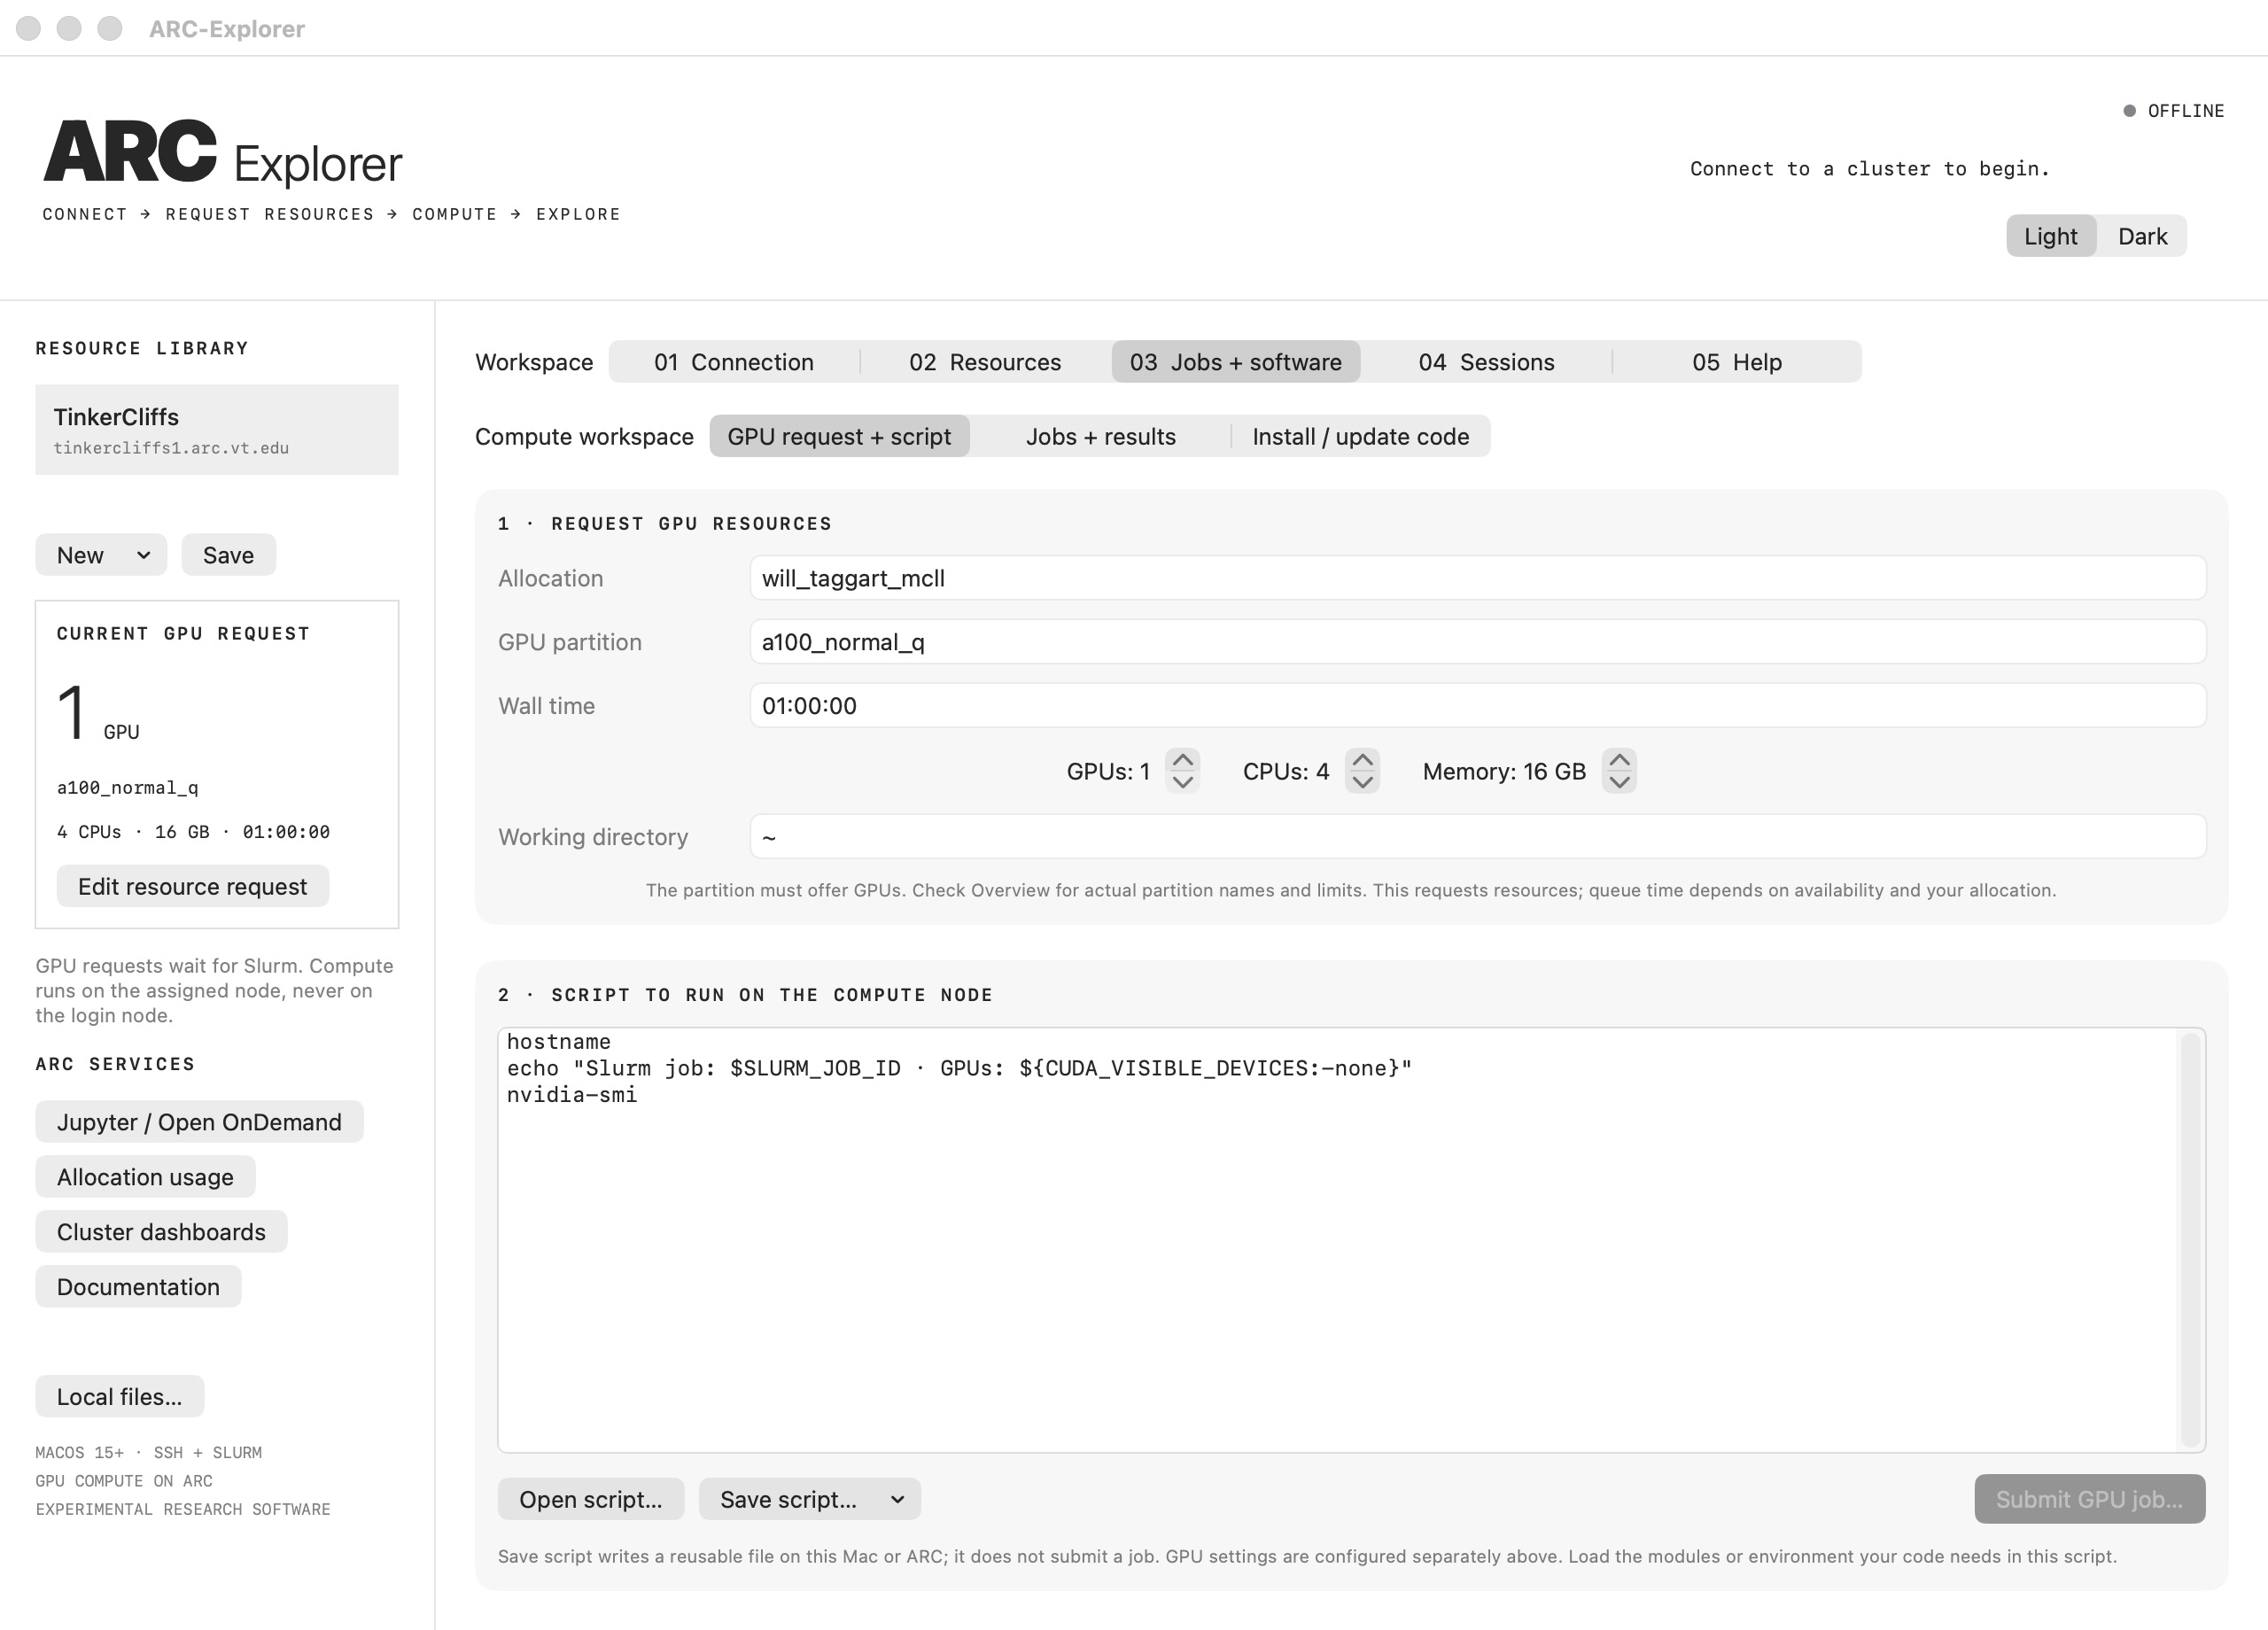
\includegraphics[width=0.78\textwidth,height=0.62\textheight,keepaspectratio]{figures/03-jobs-software.png}
\caption{Jobs + software showing explicit GPU resources and the editable script. The example script has not been submitted in this offline screenshot.}
\Description{Jobs + software showing explicit GPU resources and the editable script. The example script has not been submitted in this offline screenshot.}
\end{figure}

\section{Sessions: terminal, web applications, and tunnels}

Sessions opens to the Login Node Terminal by default. The terminal occupies the available workspace width and accepts input directly at the shell prompt. SwiftTerm supplies terminal emulation \cite{swiftterm}, connected to a local pseudo-terminal and the system SSH client, which requests a remote pseudo-terminal and an interactive login shell. Input, ANSI output, history keys, tab completion, interrupts, copying, pasting, and window-size changes follow the terminal session rather than a separate command-entry field. The scrollback limit is 5,000 lines.

The warning “Login node is not for compute intensive jobs.” appears in red directly below the terminal heading. Starting this terminal does not request a GPU allocation. It is a real shell with the user's remote permissions, not a sandbox or a restricted command catalog. Compute-intensive work belongs in a scheduled allocation. Closing the terminal closes that shell; it does not necessarily cancel independently submitted jobs or detached remote processes.

The vendored terminal implementation disables remote clipboard-read requests. Users can still deliberately paste text into the terminal. The terminal view is retained while navigating other workspace sections. Disconnecting or quitting with an active terminal requests confirmation so that an interactive shell is not discarded silently.

Web / Jupyter embeds ARC web applications through WebKit. Open OnDemand provides its own authentication, resource forms, and application lifecycle \cite{arcood}. The desktop GPU form does not automatically provision every embedded web session. A system-browser option accommodates services whose authentication or browser features do not work well inside an embedded view. Bookmarks support additional ARC services, but compatibility with every service is not guaranteed.

For an existing service on an allocated compute node, a tunnel maps a local loopback port through SSH to a user-specified compute host and remote port. Host and port inputs are validated, and the local listener binds to 127.0.0.1. The user must first start the service in the allocation and supply the appropriate URL or token. Closing the tunnel removes connectivity; it does not stop the underlying job. The application does not infer ownership or readiness of every manually specified remote service.

\begin{figure}[!htb]
\centering
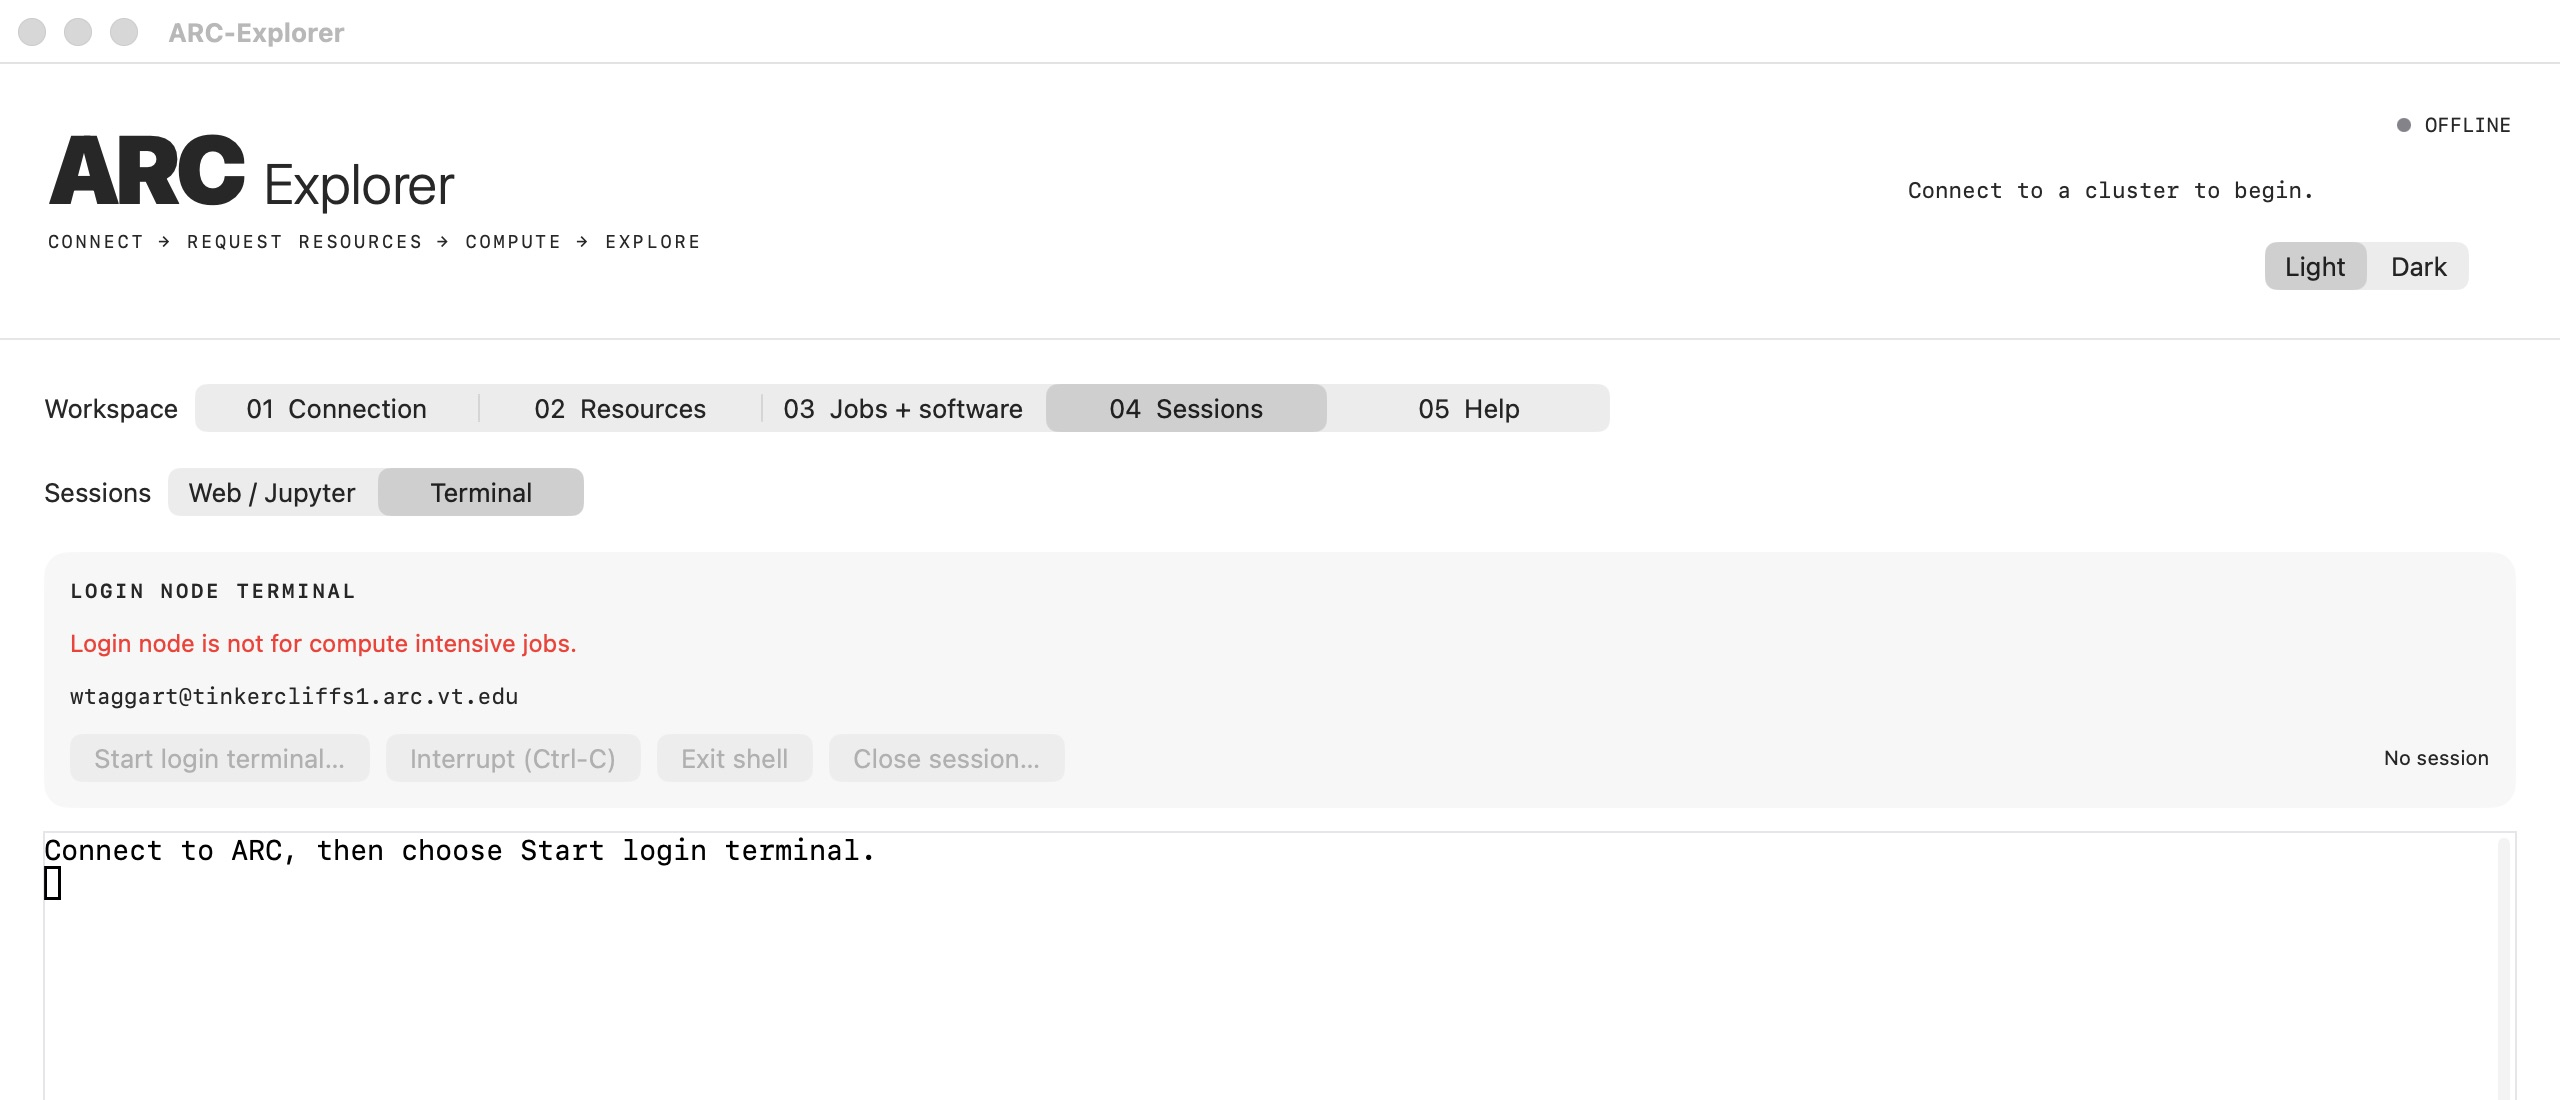
\includegraphics[width=0.78\textwidth,height=0.62\textheight,keepaspectratio]{figures/04-sessions.png}
\caption{Sessions with the full-width Login Node Terminal controls, upper terminal pane, and red compute warning. The terminal is disconnected in this capture.}
\Description{Sessions with the full-width Login Node Terminal controls, upper terminal pane, and red compute warning. The terminal is disconnected in this capture.}
\end{figure}

\section{Help: command reference and ARC-hosted language models}

The Help section combines a fixed command reference with an optional ARC-hosted LLM assistant. The command reference includes partition inspection, queue and history queries, account associations, module discovery, and storage commands. A command can be copied or placed into the GPU script editor for review. This exposes the actual command syntax and keeps execution separate from explanation.

The assistant uses ARC's documented OpenAI-compatible API \cite{arcllm}. Its base URL is configurable, with the ARC endpoint supplied by default. Available model identifiers are fetched from the service rather than presented as a permanent catalog. Access depends on the user's API key, account permissions, network access, and the models currently offered by ARC. A model identifier visible in a screenshot is a saved selection, not a claim of current availability.

A request contains the user's typed question and a general ARC-help instruction. Files, job logs, connection passwords, and private keys are not attached automatically. Responses are advice only and never execute commands. Users can nevertheless disclose information by typing it into a question, so the data boundary is determined in part by what they choose to send.

The transport requires HTTPS and refuses HTTP redirects, preventing automatic forwarding of the bearer credential to a redirected destination. API keys remain in memory unless the user explicitly saves one to macOS Keychain. Changing the API base clears the in-memory key. Requests are non-streaming, use a 120-second timeout, and request at most 4,096 output tokens. Errors are surfaced to the user; the assistant is not an autonomous troubleshooting or job-execution agent.

\begin{figure}[!htb]
\centering
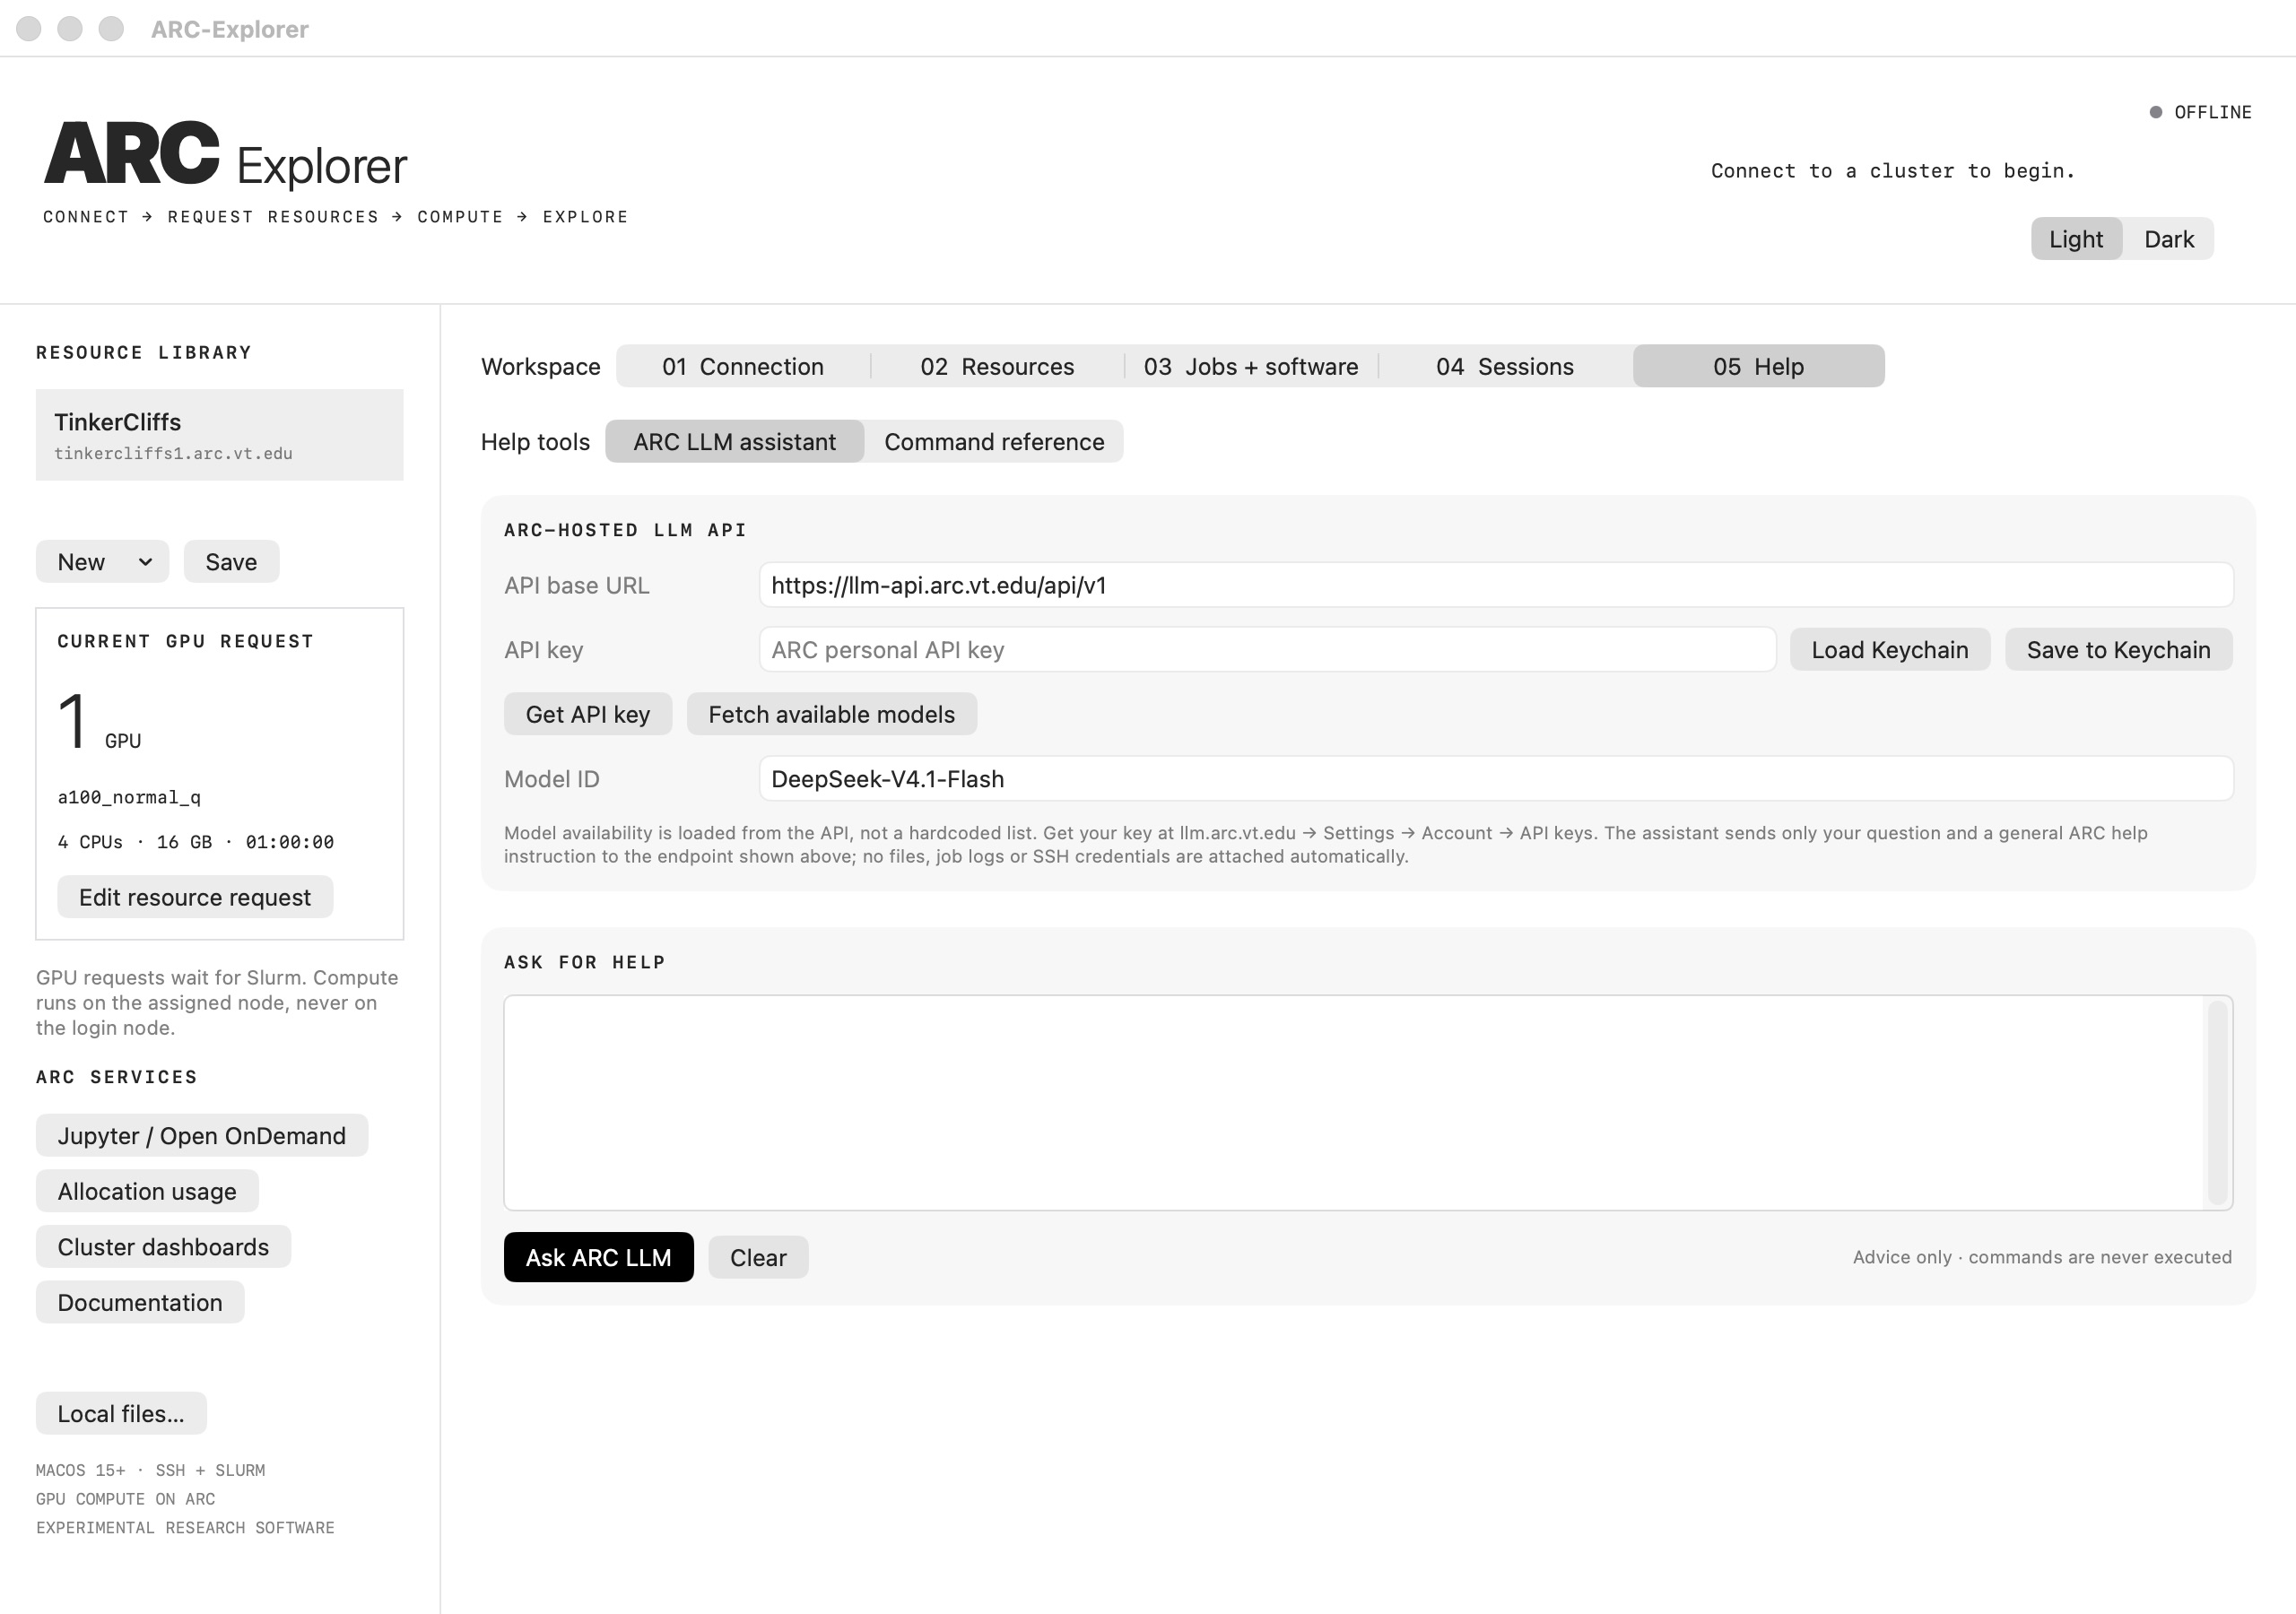
\includegraphics[width=0.78\textwidth,height=0.62\textheight,keepaspectratio]{figures/05-help.png}
\caption{Help section with the ARC API configuration, model field, and question editor. The API key is empty; no live response is claimed.}
\Description{Help section with the ARC API configuration, model field, and question editor. The API key is empty; no live response is claimed.}
\end{figure}

\section{Verification, distribution, and reproducibility}

The v0.1 release build passes 28 Python tests and two Swift terminal tests. Python coverage includes resource validation, rejection of malformed identifiers, submission through sbatch rather than login-shell script execution, ownership checks for cancellation, independent report failures, repository-update guards, transfer bounds, and remote editor conflicts. File tests exercise Unicode, byte-order marks, CRLF preservation, permission preservation, binary rejection, link rejection, exclusive creation, and cleanup after a detected save conflict.

The native tests verify login-terminal request construction without an allocation requirement and exercise a real local pseudo-terminal: interactive input, a requested terminal size of 42 rows by 140 columns, and process exit. These are targeted regression checks. They do not prove all escape-sequence behavior, SSH authentication combinations, remote policy compliance, or embedded-browser compatibility.

The five figures are captures of the application interface, all captured from the signed release build. The images are cropped to remove unused space and pointer/hover overlays. They deliberately show offline states and omit live account results and credentials. Screenshots document layout and available controls; they are not measurements of scheduler or API success. Earlier development included remote smoke checks, but this report's quantified release evidence is limited to the test suite stated above.

The source distribution includes the Swift application, remote helper, native askpass helper, icon generator, tests, build script, vendored terminal source and license, and this report in Markdown, LaTeX, and PDF. SwiftTerm is pinned to v1.20.0 with the documented clipboard-read change. The build targets arm64 and macOS 15.0; the release was built and tested on a newer macOS host, not separately runtime-qualified on every supported OS release.

The application and its helper are signed with a Developer ID Application identity and hardened runtime. The release workflow submits an archive to Apple's notarization service, staples an accepted ticket to the app, and verifies the resulting bundle before creating the downloadable ZIP. Notarization is a distribution check rather than a certification of the scientific workflow or a functional test. The release manifest records the actual notarization state and artifact checksums; source rebuilds require the builder's own signing identity and credentials for a separately notarized distribution.

\section{Limitations and future work}

ARC Explorer is experimental research software and an independent client, not an official replacement for ARC documentation or support. Partition names, command availability, API models, quotas, and site policies change. Query results depend on user permissions and may be incomplete. The interface can connect to a custom host, but the management helper assumes a compatible shell, Python 3, and Slurm environment.

The file browser is intended for small interactive operations, the editor for ordinary UTF-8 files, and the native job form for single-node GPU work. Large transfers, rich document editing, fully transactional concurrent editing, CPU-only forms, multi-node jobs, and comprehensive job-array management are outside this release. An unrestricted terminal provides flexibility but cannot prevent harmful or policy-inappropriate commands. The LLM assistant can produce incorrect advice and cannot validate resource availability on its own.

Future evaluation should include runtime tests on macOS 15, authenticated tests across each supported cluster, representative Jupyter and SSO flows, API model discovery and response tests with authorized credentials, accessibility review, and a user study of common end-to-end tasks. Potential extensions include CPU-only and multi-node forms, resumable bulk transfer, and richer accounting exports. These are proposed directions, not v0.1 capabilities.

\section{AI disclosure}

This project was created with assistance from GPT-6 Astra and Codex. AI tools assisted with implementation, debugging, testing, and drafting and formatting documentation. William Taggart directed the project. This disclosure does not imply independent human validation of every implementation detail or AI-generated statement. The references identify the primary sources used for external technical claims.

\bibliographystyle{ACM-Reference-Format}
\bibliography{references}
\end{document}
